\documentclass[11pt]{article}
\usepackage[margin=0.88in]{geometry}
\usepackage{amsmath,booktabs,graphicx,microtype,hyperref}
\hypersetup{colorlinks=true,urlcolor=blue,linkcolor=black}
\setlength{\parindent}{0pt}\setlength{\parskip}{4pt}
\title{Numerical Exhibits for All-Pass Judge Evaluation}
\author{RefEval research companion}
\date{November 2026}
\newcommand{\checkerrows}{%
Official & 40 & 208 / 209 & 52 / 31 & -12 & +9 & [5.1, 27.1] \\
Literal suffix & 35 & 200 / 217 & 52 / 31 & -16 & +5 & [0.0, 18.6] \\
Omit suffix & 41 & 189 / 197 & 52 / 37 & -11 & +4 & [-3.4, 16.9] \\
}

\newcommand{\repeatrows}{%
Original & -12 & +8 & 24 & -3 & -4 & 17 \\
Exact repeat & -14 & +6 & 24 & -3 & -4 & 17 \\
Alternative & -11 & +4 & 19 & -3 & +0 & 15 \\
}

\newcommand{\costrows}{%
JudgmentBench & 10.56 & 15.89 & -5.33 & [-5.91, -4.61] \\
Agentic coding & 11.29 & 9.57 & +1.72 & [-0.71, +3.45] \\
Deep research & 2.62 & 2.34 & +0.28 & [-0.35, +0.79] \\
}

\newcommand{\selectorsrows}{%
Deep research & 284 & 3.52 & 4.58 & 3.52 & +2.11 & +2.46 & +2.11 \\
Agentic coding & 210 & 14.29 & 14.29 & 14.29 & -0.95 & -0.95 & -0.95 \\
JudgmentBench & 1539 & 15.85 & 15.85 & 15.85 & -12.74 & -12.74 & -12.74 \\
ProfBench Critical & 114 & 8.77 & 8.77 & 9.65 & +0.00 & +0.00 & +0.88 \\
}

\newcommand{\externalrows}{%
Fixed & 1:1 & U (31.43) & U (31.43) & U (31.43) \\
Fixed & 3:1 & U (83.93) & G (41.79) & G (41.79) \\
Fixed & 1:3 & U (41.79) & U (41.79) & U (41.79) \\
Calibrated & 1:1 & G (28.04) & U (26.34) & G (28.04) \\
Calibrated & 3:1 & G (75.54) & U (62.59) & G (75.54) \\
Calibrated & 1:3 & G (36.61) & G (36.61) & G (36.61) \\
}

\begin{document}
\maketitle
\begin{table}[!htbp]
\centering\small
\caption{Upgrading the GPT judge on the original 59 common outputs. Counts separated by a slash give mini then GPT-5.5. Signed changes give GPT-5.5 minus mini. The last column is a paired 95\% percentile interval for extra false failures per 100 outputs, resampling source groups within generator and rubric-length strata.}
\begin{tabular}{lrrrrrr}\toprule
Scoring rule & Ref. passes & Correct items & Judge passes & $\Delta$FP & $\Delta$FF & 95\% per 100\\\midrule
\checkerrows\bottomrule\end{tabular}\end{table}
\begin{table}[!htbp]
\centering\small
\caption{Same answers submitted three times under the official checker. FP and FF are strong minus light counts. The third column of each family counts outputs on which the two judges disagree. Of the 59 originally eligible four-model outputs, 58 have complete GPT results across all three arms and 59 have complete Claude results.}
\begin{tabular}{lrrcrrc}\toprule &\multicolumn{3}{c}{GPT} & \multicolumn{3}{c}{Claude}\\
 & $\Delta$FP & $\Delta$FF & Disagreements & $\Delta$FP & $\Delta$FF & Disagreements\\\midrule
\repeatrows\bottomrule\end{tabular}\end{table}
\begin{figure}[!htbp]
\centering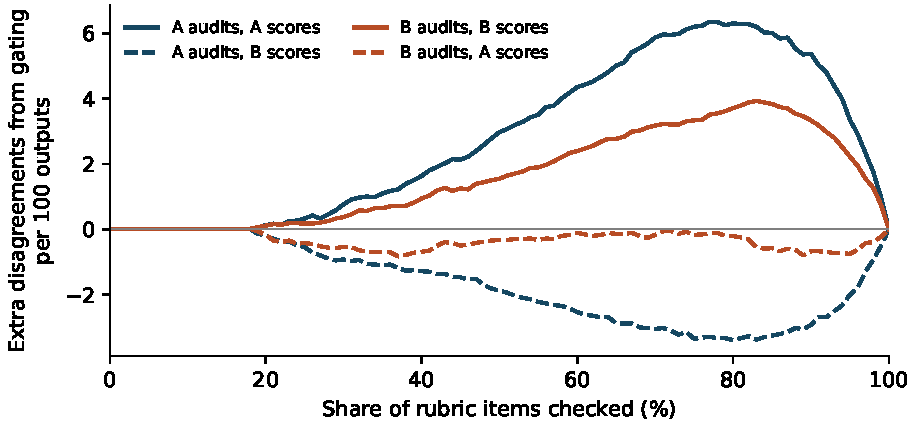
\includegraphics[width=.84\linewidth]{generated/rater_curve.pdf}
\caption{Gated minus eager disagreement under disagreement-first checking, full JudgmentBench target and GPT-5.4. Positive values favor immediate updating. Each point averages the same 31 priority orders. The dashed and solid curves of each color use identical audit answers.}\end{figure}
\begin{table}[!htbp]
\centering\small
\caption{Eager disagreements per 100 units at an opening cost of 15 criterion checks. The range shows the middle 95\% of paired order differences. The three rows use GPT-5.4, DeepSeek v4-pro and Gemini 3.1 Pro, respectively.}
\begin{tabular}{lrrrr}\toprule & SC & DF & SC minus DF & Order range\\\midrule
\costrows\bottomrule\end{tabular}\end{table}
\begin{table}[!htbp]
\centering\small
\caption{Selections evaluated out of fold at equal verdict costs. Crit., task and prod. select by criterion error, observed verdict error and product forecast. Signed pass-rate bias equals false passes minus false failures per 100 outputs.}
\begin{tabular}{lrrrrrrr}\toprule & &\multicolumn{3}{c}{Errors / 100}&\multicolumn{3}{c}{Pass-rate bias (pp)}\\
Frame & $N$ & Crit. & Task & Prod. & Crit. & Task & Prod.\\\midrule
\selectorsrows\bottomrule\end{tabular}\end{table}
\begin{table}[!htbp]
\centering\small
\caption{Judge chosen in development and weighted loss per 100 held summaries. U denotes UniEval and G denotes G-Eval. Costs are false pass to false fail. The primary test is the fixed mapping at equal costs.}
\begin{tabular}{llrrr}\toprule Mapping & Cost & Criterion & Observed task & Product\\\midrule
\externalrows\bottomrule\end{tabular}\end{table}
\end{document}
